\providecommand{\mainpath}{..} % Command to retrieve the path of the main file. It must be defined before documentclass.

\documentclass[\mainpath/main]{subfiles}
\begin{document}

\chapter{User Interfaces Design}
\label{UIDesign}

% Command to be executed after the starting of every chapter
\setmyfancystyle
% ----------------

In this chapter are shown the main \glspl{mockup} of myTaxiService, due to present the graphical user interfaces of the system for each functionality. All the \glspl{mockup} are displayed with an accurate description to prevent misunderstanding and to recall the functionality.\\

\section{Registration/Login}
When an user connects to the WS or opens the MA, the first screens is the login page. For both the versions, there is a button to redirect to the registration page, if the user is not registered yet.\\
The figure \ref{UI:loginWS} is the WS version where the registration button is made by a link on the phrase \textquotedblleft Not Registered yet? Click here\textquotedblright. At the same time the user can insert his credentials into the specific boxes.\\
The figure \ref{UI:loginMA} is the corresponding \gls{mockup} for the mobile application: at the application opening the user can inserts his credentials or clicks on the registration button.\\

\clearpage

\begin{figure}[ht!]
	\centering
	\begin{minipage}[t]{0.45\textwidth}
		\centering
		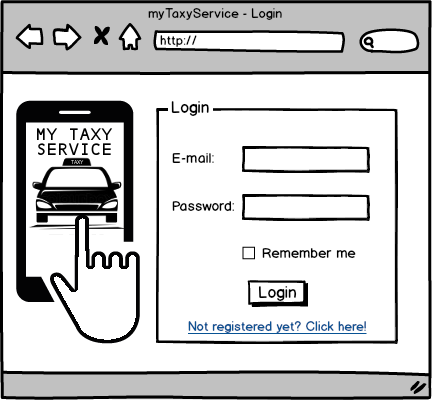
\includegraphics[width = \linewidth] {mockups/Login_WS}
		\caption{Login page into website.}
		\label{UI:loginWS}
	\end{minipage}
	\hspace{0.05 cm}
	\begin{minipage}[t]{0.45\linewidth}
		\centering
		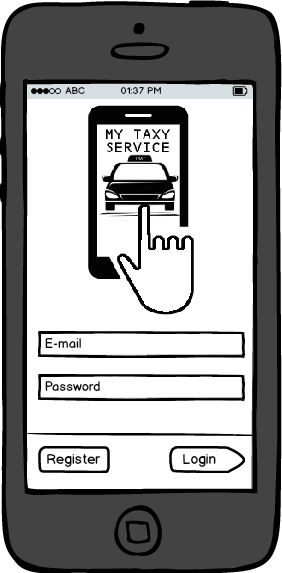
\includegraphics[height = 8cm] {mockups/Login_MA}
		\caption[Login page into mobile application.] {\scriptsize Login page into mobile application.}
		\label{UI:loginMA}
	\end{minipage}
\end{figure}

A non registered user has to enrol into the system, so he clicks on the corresponding button and he is redirected to that page. The figures \ref{UI:registrationWS} and \ref{UI:registrationMA} shows the \glspl{mockup} for this: into the \gls{ma} the box labels are written into them and disappears when the user fills in; into the \gls{ws} the labels are shown near the corresponding one.\\

\begin{figure}[ht!]
	\centering
	\begin{minipage}[t]{0.45\textwidth}
		\centering
		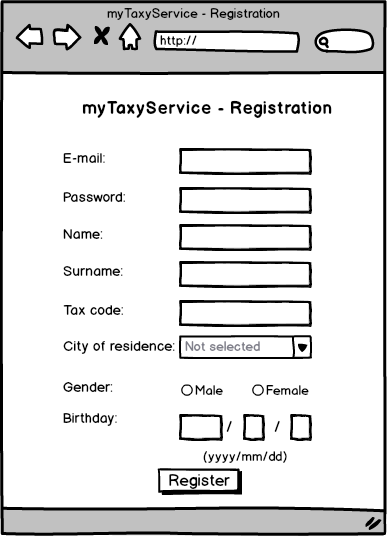
\includegraphics[width = \linewidth] {mockups/Registration_WS}
		\caption{Registration page into website.}
		\label{UI:registrationWS}
	\end{minipage}
	\hspace{0.05 cm}
	\begin{minipage}[t]{0.45\linewidth}
		\centering
		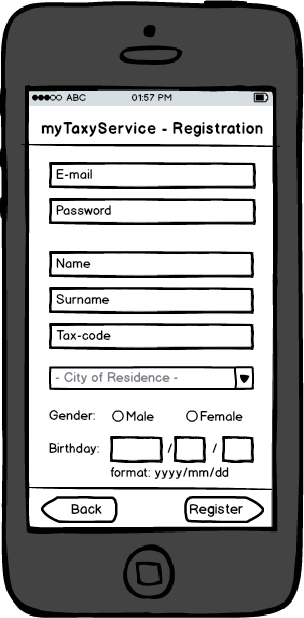
\includegraphics[height = 8cm] {mockups/Registration_MA}
		\caption[Registration page in mobile application.] {\scriptsize Registration page in mobile application.}
		\label{UI:registrationMA}
	\end{minipage}
\end{figure}







%End of chapter
\end{document}